\chapter{Professor UI Requirements}

    \begin{section}{Professor Clicks on Side or Top Navigation Buttons}
        Description: While on any page containing navigation links in the side or top bars, the professor clicks on a nav link \newline
        Primary Actors: Professor \newline
        Steps:
        \begin{enumerate}
            \item{The professor is logged into any of the main pages containing nav links}
            \item{The professor clicks on any link}
        \end{enumerate}
        Successful Post Conditions:
        \begin{itemize}
          \item{The professor is directed to the page intended by the link}
        \end{itemize}
        Exceptional Condition:
        \begin{itemize}
           \item{The professor is already on the page of the link they are clicking - nothing happens and the page does not change.}
        \end{itemize}
    \end{section}
    
    \begin{section}{Professor Clicks on the Assignment Submission Ticker}
        Description: From the main landing page the professor clicks on the assignment submission ticker \newline 
        Primary Actor: Professor \newline
        Steps:
        \begin{enumerate}
            \item{The professor is on the main page after login}
            \item{The professor clicks on the Assignment Submission Ticker Pane}
        \end{enumerate}
        Successful Post Condition:
        \begin{itemize}
            \item{The professor is redirected to a larger detailed view with a time directed log of student submission stats for assignments the professor has created, or is linked to through class ownership}
        \end{itemize}
        Exceptional Post Condition:
        \begin{itemize}
            \item{The professor has no submissions in his feed - he is directed to the log but is not shown any information}
        \end{itemize}
    \end{section}
    
    \begin{section}{Professor Clicks on the Class or Student Ticker}
        Description: From the main landing page the professor clicks on enrolled student/ class ticker pane \newline
        Primary Actor: Professor \newline
        Steps:
        \begin{enumerate}
            \item{The professor is on the main page after login}
            \item{The professor clicks on the enrolled student/ class ticker pane}
        \end{enumerate}
        Successful Post Condition:
        \begin{itemize}
            \item The professor is redirected to a larger detailed view with the option to sort by class or student name to display stats pertaining to course enrollment and individual student assignment histories
        \end{itemize}
    \end{section}
    
    \begin{section}{Professor Clicks to Expand the Assignment Creation Sandbox}
        Primary Actor: Professor \newline
        Steps:
        \begin{enumerate}
        \item{The professor is on the main page after login} 
        \item{The professor clicks to expand the assignment creation sandbox}
        \end{enumerate}
        Successful Post Condition:
        \begin{itemize}
        \item{The professor is taken to the assignment creation page and any potential diagrams or questions created in the sandbox are stored and transferred to the assignment creation window}
        \end{itemize}
    \end{section}
    
    \newpage
    \iffalse
    \begin{section}{Professor View}
        \begin{figure}[h!]
                \centerline{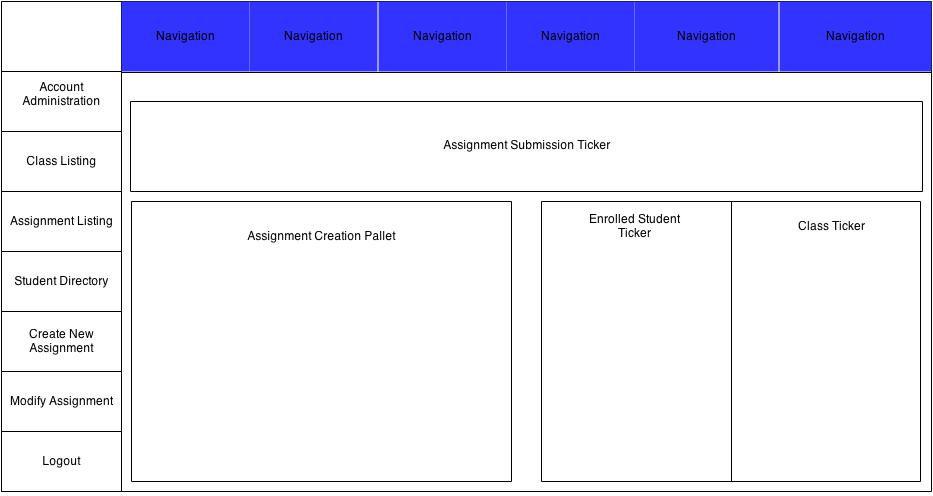
\includegraphics[width=13cm]{ProfessorView.jpg}}
                \caption{Professor's User Interface}
        \end{figure}
    \end{section}
    \newpage

    \begin{section}{Create}
        \begin{figure}[h!]
                \centerline{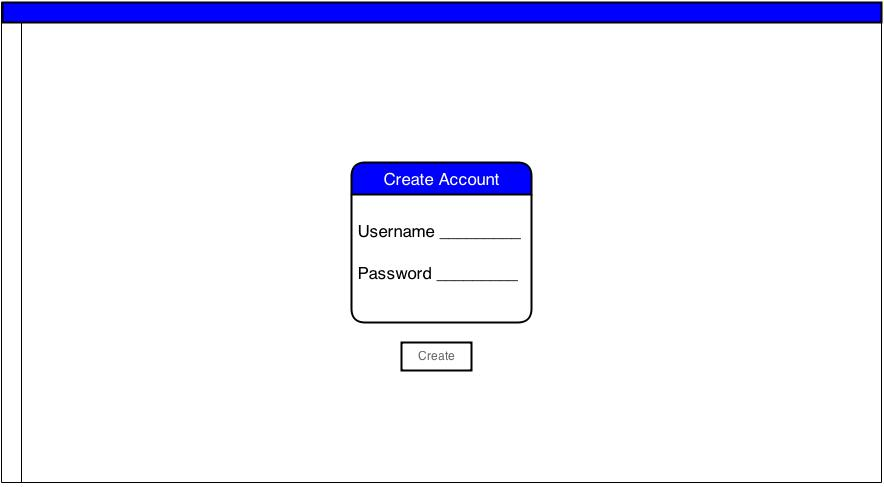
\includegraphics[width=13cm]{UICreate.jpg}}
                \caption{User Interface to create question}
        \end{figure}
    \end{section}
    \newpage
    \begin{section}{Login}
        \begin{figure}[h!]
                \centerline{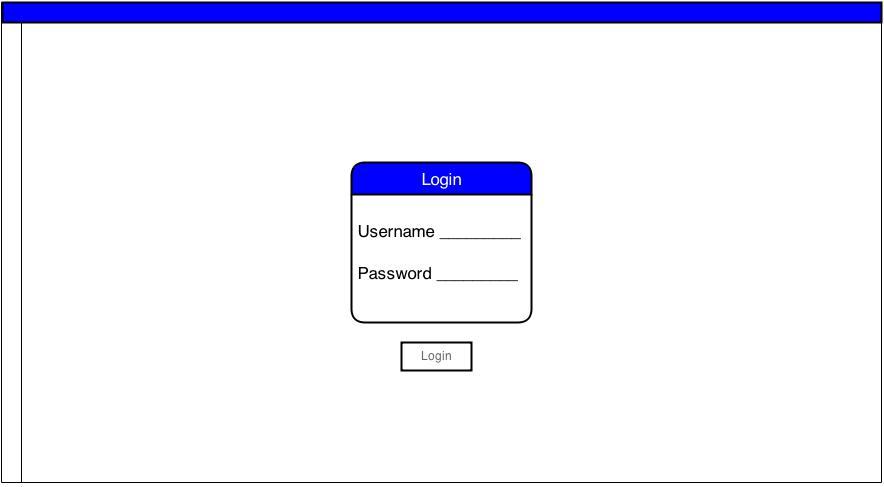
\includegraphics[width=13cm]{UILogin.jpg}}
                \caption{Login User Interface}
        \end{figure}
        \end{section}
        \newpage
        \begin{section}{Student}
        \begin{figure}[h!]
                \centerline{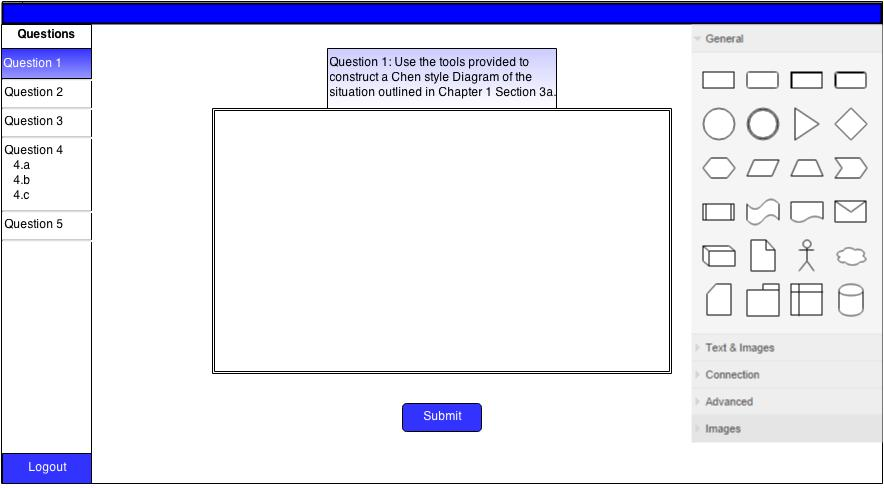
\includegraphics[width=13cm]{uistudent.jpg}}
                \caption{User Interface for the student}
        \end{figure}
  
    \end{section}

      \fi


